\chapter{Existing System Analysis and State of the Art}

\section*{Introduction}
\addcontentsline{toc}{section}{Introduction}

The present chapter establishes the technical and operational foundations upon which the FiberGate solution was designed. It is organized into four progressive analytical sections, each narrowing the focus from macro-level infrastructure context to specific tooling limitations that motivated this project.

The first section introduces the FTTX network architecture and the role of the Access Point (PAR) within the GPON hierarchy, providing the engineering vocabulary necessary to understand the workflows documented in subsequent sections. The second section describes the operational workflows of the Guichet OI unit in precise, step-by-step terms derived from the official operational guidelines and internal distribution procedures. The third section analyzes the structural bottlenecks and systemic limitations that those workflows produce at scale. The fourth section surveys the state of the art in the three technology domains relevant to the proposed solution: Robotic Process Automation, Document Artificial Intelligence and multimodal learning, and enterprise web application architectures. The chapter concludes with a comparative positioning of the selected technologies against available alternatives.

\section{FTTX Technology and PAR Engineering Fundamentals}

The following subsections introduce the FTTX passive optical network paradigm, the specifics of its deployment in France under the two Orange operator models, and the engineering process associated with PAR localisation that constitutes the primary value-adding activity of the Guichet OI unit.

\subsection{FTTX Principles and GPON Network Hierarchy}

Fiber to the X (FTTX) is a collective term designating any broadband network architecture that uses optical fiber as the primary transmission medium for part or all of the last-mile connection between a telecommunications operator and a subscriber. The X suffix denotes the fiber termination point: the home (FTTH), the office (FTTO), the building (FTTB), or the antenna (FTTA). In each variant, the optical fiber carries data as modulated light pulses over glass or plastic strands, enabling theoretical throughput in the range of gigabits per second with negligible signal degradation over distances of several kilometers.

The passive optical network (PON) paradigm underpins all FTTX deployments in France. In a PON, a single Optical Line Terminal (OLT) located at the central office drives multiple subscriber endpoints through a tree of passive optical splitters. No active electronic components exist between the OLT and the Optical Network Units (ONUs) at the subscriber premises. France's dominant standard is GPON (Gigabit-capable Passive Optical Network), defined under ITU-T G.984.1, which supports downstream rates of up to 2.488 Gbps shared among 64 or 128 subscribers on a single PON port.

The FTTX deployment model in France follows a hierarchical node structure progressing from the central office to the optical distribution frame (NRO/ODF), then to the sub-distribution node (SRO), then to the building-level access point (PAR), and finally through the subscriber box (PBO) to the terminal optical socket (PTO) inside the residential unit. The diagram below illustrates this hierarchy and positions the PAR node within it.

\begin{figure}[H]
  \centering
  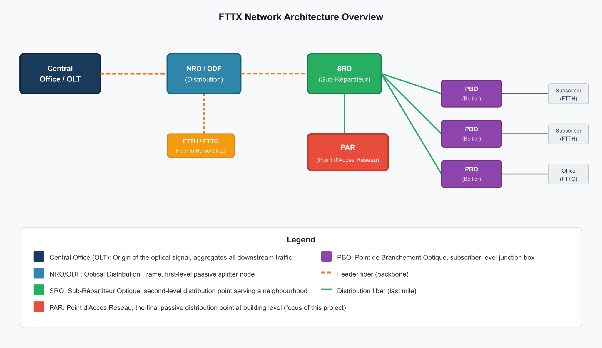
\includegraphics[width=0.52\textwidth,max width=\textwidth]{images/image9.png}
  \caption{FTTX network hierarchy illustrating the GPON node chain from OLT to subscriber PTO}
  \label{fig:image9}
\end{figure}

\subsection{Fiber Infrastructure Deployment in France}

France's national fiber deployment program, Plan France Tres Haut Debit, targets universal very high-speed broadband coverage. Orange, as the incumbent operator and the largest infrastructure operator, has deployed fiber to over 38 million premises, covering approximately 80 percent of the French population. This deployment is organized under two distinct operator models that directly shape the operational context of the Guichet OI unit.

\begin{figure}[H]
  \centering
  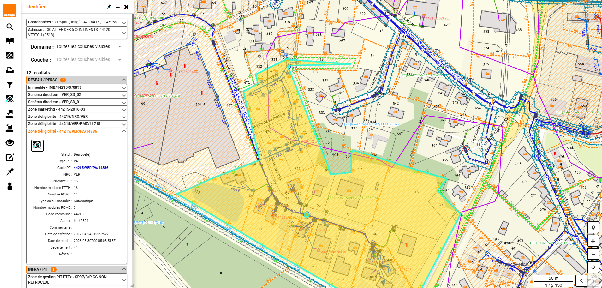
\includegraphics[width=0.52\textwidth,max width=\textwidth]{images/image10.png}
  \caption{Fiber Infrastructure In France}
  \label{fig:image10}
\end{figure}

Under the OSA model (Operateur Service Activateur), Orange assumes simultaneously the role of infrastructure operator and service provider. All connection requests processed under the OSA model are managed by the Amaris team at the Guichet OI unit and constitute the exclusive scope of the automation solution developed in this project. Under the OCC model (Operateur Commercial Client), Orange operates the physical infrastructure while a third-party operator sells and activates services over it. OCC requests follow a distinct processing path and are explicitly excluded from the automation workflows, as reflected in the filtering logic of Agent 3.

The infrastructure is organized across three deployment zones: the feeder zone connecting the NRO to the SRO over distances of 2 to 5 km; the distribution zone connecting the SRO to the PAR over distances of 200 to 500 meters; and the drop zone connecting the PAR to the subscriber over 10 to 50 meters of indoor cable. At the building level, the fiber terminates at the PAR, which constitutes the critical handoff point between the operator's network and the internal building wiring.

\begin{table}[H]
  \centering
  \caption{FTTX node types and their operational relevance to the Guichet OI unit}
  \renewcommand{\arraystretch}{1.0}
  \footnotesize
  \begin{tabularx}{\textwidth}{|>{\raggedright\arraybackslash}p{2.3cm}|X|X|X|}
    \hline
    \textbf{Node} & \textbf{Location} & \textbf{Technology} & \textbf{Role in Guichet OI Context} \\ \hline
    OLT & Central office & Active GPON equipment & Data origin; no direct role in Guichet OI processing \\ \hline
    NRO / ODF & Street cabinet & Passive splitter 1:4 or 1:8 & First-level distribution node \\ \hline
    SRO & Neighbourhood cabinet & Passive splitter 1:8 or 1:16 & Sector-level distribution \\ \hline
    PAR & Building entrance & Passive splice or connector box & Primary focus: engineering and localisation workflow \\ \hline
    PBO & Floor or facade box & Passive connector panel & Drop-cable junction, subscriber-facing \\ \hline
    PTO & Inside apartment & Optical socket & Subscriber termination point \\ \hline
  \end{tabularx}
\end{table}

\subsection{PAR Engineering Processes and Operational Performance Indicators}

The Point d'Acces Reseau (PAR) is the passive optical distribution node located at the entry of a building or at the boundary of a land plot. Its engineering involves determining the physical location, type, capacity, and construction requirements for this node, a process referred to as PAR localisation. The Guichet OI unit manages this process for every new real estate fiber connection request submitted by engineering offices (bureaux d'etudes) acting on behalf of property developers.

PAR localisation is performed through one of two methods depending on project type and technical complexity. The first method, online localisation, applies to standard residential buildings and small operations (petites operations immobilieres) where the network topology is already documented. The consultant uses the GEORESO tool to identify an existing or suitable PAR position and produces a chartered location plan. The second method, CAFF-based localisation, applies to complex projects including ZAC developments, large collective housing, and any project requiring physical network verification. A Chef d'Affaire Fibre is dispatched to the site via a POI created in GEDAFFAIRES, produces a chartered PAR plan, and transmits it back to the Guichet OI unit.

\begin{figure}[H]
  \centering
  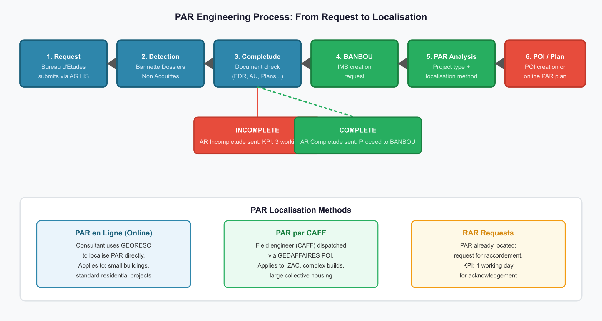
\includegraphics[width=0.52\textwidth,max width=\textwidth]{images/image11.png}
  \caption{End-to-end PAR engineering process: method selection, execution, and plan transmission}
  \label{fig:image11}
\end{figure}

The Guichet OI unit operates under a set of contractually defined key performance indicators that govern response times at each stage of the PAR workflow. These KPIs are monitored by the Service Delivery Manager and reported to Orange France. Failure to meet them constitutes a service-level breach with commercial consequences.

\begin{table}[H]
  \centering
  \caption{Operational KPIs governing the Guichet OI PAR France unit}
  \renewcommand{\arraystretch}{1.0}
  \footnotesize
  \begin{tabularx}{\textwidth}{|X|X|X|X|}
    \hline
    \textbf{KPI} & \textbf{Trigger Event} & \textbf{Target} & \textbf{Pre-Automation Status} \\ \hline
    AR Completude / Incompletude & New PAR request detected in bannette & 3 working days & Frequently met but at high human cost \\ \hline
    CAFF return treatment & CAFF return email received in shared mailbox & 1 working day & Frequently breached for after-hours arrivals \\ \hline
    POI validation processing & AGILIS POI confirmation email received & Same day & 15 to 20 minutes per email, approximately 15 per day \\ \hline
    Daily task distribution & Full PAR France file available at 09:50 & Before 10:30 & 30 to 45 minutes of manual Excel work \\ \hline
    GOLP completeness review & Go Lancement Projet request in bannette & 3 working days & Met with sustained manual effort \\ \hline
  \end{tabularx}
\end{table}

\section{Operational Workflows of the Guichet OI Unit}

The Guichet OI PAR France unit processes real estate fiber connection requests through a structured four-stage workflow defined in the official Orange operational guidelines. The four stages are: Stage 1, Demande de localisation de PAR; Stage 2, Go lancement projet; Stage 3, Prise en compte des INOI; and Stage 4, Demande de RAR. Each stage defines its own completeness criteria, acknowledgement communications, and AGILIS state transitions. All requests enter the system through the AGILIS platform, where engineering offices deposit connection requests along with their mandatory supporting documents.

\subsection{End-to-End Workflow Overview and Tool Landscape}

\begin{figure}[H]
  \centering
  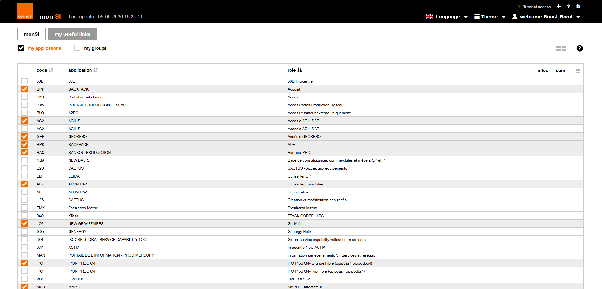
\includegraphics[width=0.52\textwidth,max width=\textwidth]{images/image12.png}
  \caption{Guichet OI: PAR France Tools}
  \label{fig:image12}
\end{figure}

The nine tools constituting the operational environment are: AGILIS for request management; SharePoint for the SUIVI tracking list and the Full PAR France Excel file; Microsoft Planner for task assignment; GEDAFFAIRES for CAFF communication; GEORESO for online PAR localisation; BANBOU for IMB record creation; OPTIMUM for IMB-to-PAR mapping and convention validation; ALCATRAZ for geodetection of fiber versus copper versus RIP infrastructure; and ELIMAP for geographic visualization. The absence of any integration layer between these tools means that every inter-system data transfer is a manual operation performed by the consultant.

\begin{figure}[H]
  \centering
  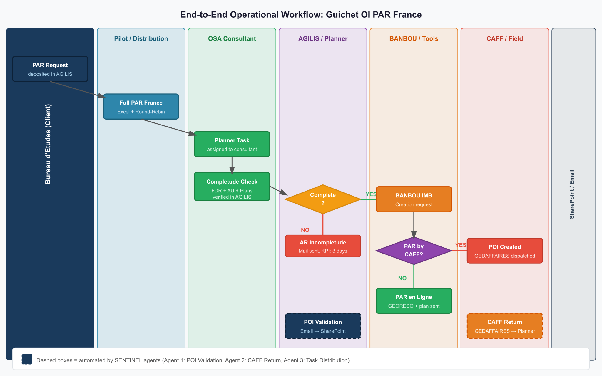
\includegraphics[width=0.52\textwidth,max width=\textwidth]{images/image13.png}
  \caption{End-to-end workflow swim-lane diagram covering all four stages and the nine operational tools}
  \label{fig:image13}
\end{figure}

\subsection{Task Distribution and Workload Characterization}

Task distribution is the responsibility of the Pilot, a dedicated senior consultant who manages the daily allocation of incoming requests to the 15 OSA consultants. The distribution process begins each morning when the Full PAR France Excel file becomes available on SharePoint at approximately 09:50. The Pilot executes the following four-step sequence manually each working day.

In the first step, the Pilot extracts data by selecting all visible rows in the Bannette Dossiers Non Acquittes filtered by Plateau equal to AMAPERF, Type de dossier equal to Projet Guichet PAR, and Categorie equal to OSA, then performs a manual copy-paste into an Excel workbook. In the second step, the Pilot downloads two Microsoft Planner exports and applies XLOOKUP and VLOOKUP formulas to determine whether each dossier already has an active Planner task and, if so, which consultant is assigned. In the third step, each row is classified by request type and assigned according to the applicable routing rule. Nouvelle Demande rows are assigned using a rotating list of the 15 consultants, while Retour Completude, RAR, and Go Lancement Projet rows are routed back to the consultant who handled the initial request under a continuity-of-treatment principle. In the fourth step, the Pilot creates a Planner task for each assigned row, populating the reference number, consultant name, request type, compartment, priority, due date, and a link to the internal SUIVI tracking list.

\begin{figure}[H]
  \centering
  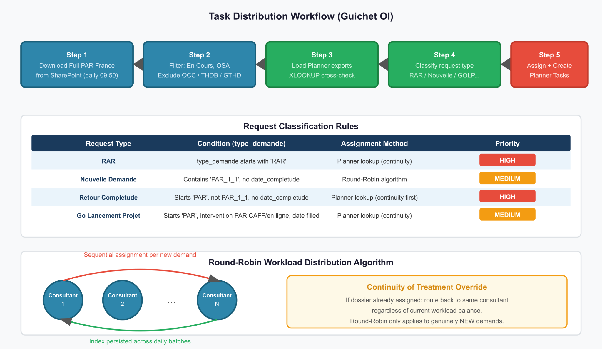
\includegraphics[width=0.52\textwidth,max width=\textwidth]{images/image14.png}
  \caption{Manual task distribution workflow: four-step sequence from Excel extraction to Planner task creation}
  \label{fig:image14}
\end{figure}

\subsection{LOC PAR Processing: Completeness Verification and Localization}

Once a task is assigned via Planner, the consultant processes the corresponding dossier in AGILIS. The LOC PAR workflow (localisation du PAR) is the most technically complex individual task in the unit and constitutes the primary value-adding activity performed by each consultant. The workflow begins with detection of the incoming request in the Bannette Dossiers Non Acquittes, followed by qualification of the request type. The first substantive step is the completeness analysis, during which the consultant examines all attached documents against the mandatory checklist.

\begin{table}[H]
  \centering
  \caption{Mandatory and optional documents for PAR location request completeness assessment}
  \renewcommand{\arraystretch}{1.0}
  \footnotesize
  \begin{tabularx}{\textwidth}{|>{\raggedright\arraybackslash}p{2.3cm}|X|X|X|}
    \hline
    \textbf{\#} & \textbf{Document} & \textbf{Status} & \textbf{Conformity Criteria} \\ \hline
    1 & Fiche de Renseignements & Mandatory & Digital format; all required fields filled; tables 1 and 2 present where applicable \\ \hline
    2 & Autorisation d'Urbanisme (PC, PA, DP, AC, AT) & Mandatory if AU number indicated in FDR & Valid AU type; Certificat d'Urbanisme and Permis de diviser are not valid \\ \hline
    3 & Plan de masse & Mandatory & Readable; buildings and lots coherent with FDR; identified on plan \\ \hline
    4 & Plan de situation & Mandatory & Parcel circled or indicated; scale sufficient for geographic identification \\ \hline
    5 & Mandat & Mandatory if mandate box checked in FDR & Client signature required; cabinet conseil signature not required \\ \hline
    6 & Plan de la servitude & Mandatory if enclosed parcel & Servitude shown on plan; signed document not required \\ \hline
    8 & Plan annote d'un PAR souhaite & Optional & Informational only; no conformity requirement \\ \hline
    9 & Certificat d'adressage & Optional at Stage 1; mandatory at Stage 3 & Official certificate or BAN screenshot with certified address \\ \hline
  \end{tabularx}
\end{table}

If the dossier is complete, the consultant sends the AR Completude acknowledgement via the MSURVEY system, marks the dossier as complete in AGILIS, and proceeds to IMB record creation in BANBOU. If incomplete, an AR Incompletude email listing all identified deficiencies is sent, and all issues must be logged simultaneously to avoid cumulative refusals in subsequent submissions. Following completeness confirmation and IMB creation, the consultant determines the PAR localisation method based on project type and executes either an online localisation using GEORESO or a CAFF-based localisation through GEDAFFAIRES and the FINOI tool.

\subsection{POI Validation Workflow}

When a consultant creates a POI of type Localiser le PAR through the FINOI tool, the AGILIS system automatically generates a confirmation email and dispatches it to the shared mailbox. This email contains six structured identifiers: the AS number, the OEIE reference, the Affaire code, the Etablissement name, the PC code, and the type\_demande\_POI.

\begin{figure}[H]
  \centering
  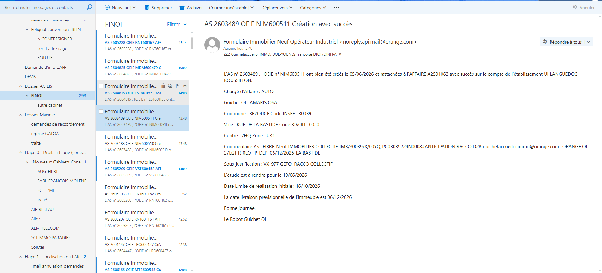
\includegraphics[width=0.52\textwidth,max width=\textwidth]{images/image15.png}
  \caption{FINOI Mailbox for POIs}
  \label{fig:image15}
\end{figure}

\subsection{CAFF Returns Processing Workflow}

When a CAFF completes field work and transmits a response through the GedAffaires platform, a notification email is automatically dispatched to the shared mailbox. The email subject line contains the OEIE reference that uniquely identifies the dossier. The operational KPI for CAFF return processing mandates acknowledgement, routing to the responsible consultant, and action within one working day of receipt.

\begin{figure}[H]
  \centering
  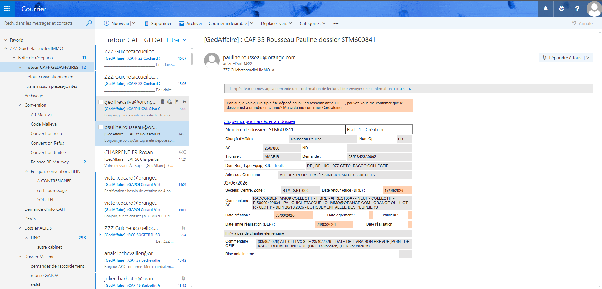
\includegraphics[width=0.52\textwidth,max width=\textwidth]{images/image16.png}
  \caption{retour CAFF GEDAFFAIRES Mailbox for CAFF Returns}
  \label{fig:image16}
\end{figure}

Prior to automation, this KPI was systematically breached for three structural reasons. First, returns arriving after 17:00 were not processed until the following morning, consuming half the KPI window before any action was taken. Second, the responsible consultant was not immediately identifiable without manually cross-referencing the OEIE code in the SUIVI tracking sheet. Third, no Planner task was automatically created to drive the follow-up action, meaning the return could remain acknowledged but untracked within the team's task management system.

\begin{table}[H]
  \centering
  \caption{Pre-automation CAFF return failure modes and their operational impacts}
  \renewcommand{\arraystretch}{1.0}
  \begin{tabularx}{\textwidth}{|X|X|}
    \hline
    \textbf{Failure Mode} & \textbf{Operational Impact} \\ \hline
    Missed evening returns & Return arrives after 17:00; not processed until the following morning; half the one-day KPI budget consumed before any action is initiated \\ \hline
    Delayed assignment identification & Responsible consultant not immediately visible; inbox monitor must open SUIVI, look up the PC code, then forward via Teams \\ \hline
    Untracked treatments & Even when the handoff occurs promptly, the absence of a Planner task means the treatment is not driven by the consultant's task board or visible in the Pilot's weekly review \\ \hline
    Volume spikes & Multiple CAFF returns arriving simultaneously overwhelm manual routing capacity; assignment quality degrades under concurrent load \\ \hline
  \end{tabularx}
\end{table}

\section{Process Analysis: Bottlenecks and Systemic Limitations}

The four workflows described in the preceding section are not operationally independent. They are temporally chained such that a delay in any upstream step propagates as a compounding constraint on all downstream steps. The task distribution workflow must complete before consultants can begin LOC PAR processing; the BANBOU IMB creation step within LOC PAR must complete before POI validation is possible; and CAFF returns can only be routed once the SUIVI SharePoint list correctly reflects the consultant assignment established during distribution.

This chaining creates a structural amplification effect. A 30-minute delay in the morning distribution routine defers the start of processing for all 15 consultants simultaneously, injecting a minimum of 450 consultant-minutes of latency at the head of every working day. When combined with the per-email overhead of POI validation processing, the total mechanical overhead extracted from analytical work across the team is substantial and quantifiable.

\begin{figure}[H]
  \centering
  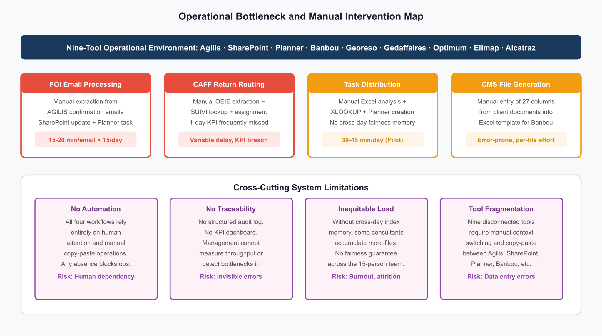
\includegraphics[width=0.52\textwidth,max width=\textwidth]{images/image17.png}
  \caption{Bottleneck map identifying the location, time cost, and automation potential of each manual intervention point}
  \label{fig:image17}
\end{figure}

\begin{table}[H]
  \centering
  \caption{Quantified manual bottlenecks in the OSA sub-team}
  \renewcommand{\arraystretch}{1.0}
  \footnotesize
  \begin{tabularx}{\textwidth}{|X|X|X|X|X|}
    \hline
    \textbf{Bottleneck} & \textbf{Time Cost} & \textbf{Daily Volume} & \textbf{Total Daily Loss} & \textbf{Automation Potential} \\ \hline
    POI email processing & 15 to 20 minutes per email & Approximately 15 emails & Approximately 4.5 hours & High (regex extraction and webhook dispatch) \\ \hline
    CAFF return routing & Variable; KPI breach risk & 5 to 10 returns & KPI compliance at risk & High (regex on subject line and SUIVI lookup) \\ \hline
    Task distribution (Pilot) & 30 to 45 minutes per batch & 1 batch per day & 30 to 45 minutes per day & High (Excel pipeline and Planner API) \\ \hline
    CMS file generation & Approximately 20 minutes per file & 8 files per consultant & Approximately 40 hours total & High (AI field extraction) \\ \hline
    Completude document check & 15 to 30 minutes per dossier & 112 files per day & Approximately 28 hours total & Medium (AI document classification) \\ \hline
  \end{tabularx}
\end{table}

Beyond the quantifiable time losses documented above, the current operating model exhibits four cross-cutting structural limitations that cannot be resolved through individual consultant performance improvement alone.

The first limitation is the absence of any automation layer. All four core workflows depend entirely on human attention and manual execution. Any absence, schedule conflict, or cognitive fatigue directly reduces team throughput. The system has no self-healing capability: a missed email is a missed KPI with no recovery mechanism.

The second limitation is the absence of traceability. No structured audit log exists for the actions performed on any dossier outside of manual AGILIS comment entries made by consultants. The Service Delivery Manager and the Pilot have no real-time visibility into which dossiers are in progress, which are blocked, or which KPIs are at risk.

The third limitation is inequitable workload distribution. Without a cross-day assignment memory, the round-robin rotation resets each morning, allowing cumulative imbalances to develop over weeks. Some consultants systematically carry more complex dossiers than others, a pattern that is invisible to management without manual count analysis.

The fourth limitation is tool fragmentation and error propagation. The nine-tool environment requires consultants to maintain context across disconnected systems. A transcription error in a PC code entered in SharePoint propagates to the Planner task, to the DEVISEUR decompte, and potentially to the GEDAFFAIRES POI, creating a chain of corrections that can take hours to unwind and that leaves no audit trace of the original error.

\section{State of the Art}

Sections~2.1 to~2.3 constituted the \textit{étude de l'existant}: a diagnosis of the operational system, its workflows, and its structural bottlenecks. The present section shifts register to the \textit{état de l'art} --- a review of the academic and industrial literature that grounds the technology selections made in Chapter~3. The two blocks answer different questions: the former establishes \emph{what must be solved}, the latter establishes \emph{what the field offers to solve it}. The boundary between them is deliberate, and the institutional option of promoting this section into a standalone chapter is left open pending validation with the academic supervisor.

The following subsections survey the literature across three technology domains directly relevant to the FiberGate solution: Document Artificial Intelligence and multimodal learning models, Robotic Process Automation and intelligent automation frameworks, and enterprise web application and cloud architecture patterns. Each subsection concludes with a positioning of the selected technology relative to the evaluated alternatives.

\subsection{Document Artificial Intelligence and Multimodal Models}

Document Artificial Intelligence refers to the set of techniques enabling automated understanding of document content, encompassing layout, typography, form fields, tables, stamps, and handwritten annotations. The LOC PAR completeness verification task represents a canonical Document AI problem: a consultant must identify the class of each attached document and extract specific field values from it, a process currently requiring 15 to 30 minutes per dossier and exhibiting error rates correlated with consultant workload and fatigue.

Three principal families of approach are documented in the state of the art. Text-only models such as BERT and LayoutLMv1 operate exclusively on the OCR-extracted text stream, ignoring spatial layout and visual page structure. They are adequate for digitally authored documents with consistent formatting but fail on scanned administrative forms where the position of a value on the page constitutes an independent semantic signal. Vision-only models such as Donut (Kim et al., 2022) treat the document as a pure image and perform classification or extraction through visual processing alone. Donut is notable for its end-to-end approach bypassing OCR entirely, using a Swin Transformer encoder and a BART-style autoregressive decoder. However, its sequential generation makes it significantly slower than encoder-only architectures and prone to producing plausible-but-incorrect text for fields with visually similar contexts.

Multimodal models such as LayoutLMv2, LayoutLMv3, and UDOP jointly process text tokens, layout coordinates expressed as bounding boxes, and image patches in a single unified transformer architecture. LayoutLMv3 (Huang et al., 2022) was selected for the FiberGate AI Service on the basis of the most favorable balance of parameter count (125 million), GPU memory requirement (7 GB), and benchmark performance within the hardware constraints of this project. Its key architectural innovation is the replacement of the cross-attention fusion mechanism of LayoutLMv2 with a unified self-attention mechanism processing all three modalities in a single stream, reducing parameter count by a factor of 3.4 relative to LayoutLMv2 while improving downstream performance on standard document understanding benchmarks.

\begin{table}[H]
  \centering
  \caption{Open-source document AI models evaluated for the FiberGate AI Service}
  \renewcommand{\arraystretch}{1.0}
  \footnotesize
  \begin{tabularx}{\textwidth}{|X|X|X|X|X|X|}
    \hline
    \textbf{Model} & \textbf{Input Modalities} & \textbf{Parameters} & \textbf{VRAM} & \textbf{Licence} & \textbf{Selection Outcome} \\ \hline
    LayoutLMv1 (2020) & Text and layout & 160M & 6 GB & MIT & Rejected: no image modality \\ \hline
    LayoutLMv2 (2021) & Text, layout, and image & 426M & 18 GB & MIT & Rejected: memory cost prohibitive for available hardware \\ \hline
    LayoutLMv3 (2022) & Text, layout, and image & 125M & 7 GB & CC-BY-NC & Selected: unified attention mechanism, balanced cost-performance ratio \\ \hline
    LiLT (2022) & Text and layout only & 250M & 7 GB & MIT & Rejected: no image modality \\ \hline
    Donut (2022) & Image only & 200M & 5 GB & MIT & Rejected: seq2seq generation too slow; no OCR layer \\ \hline
    UDOP (2023) & Text, layout, and image & 742M & 24 GB & MIT & Rejected: 24 GB VRAM requirement exceeds available hardware \\ \hline
  \end{tabularx}
\end{table}

\subsection{Robotic Process Automation: Approaches and Frameworks}

Robotic Process Automation (RPA) refers to the use of software agents that emulate human interactions with user interfaces, application programming interfaces, or communication protocols to automate rule-based, repetitive digital tasks. Agostinelli et al. (2023) define RPA as the deployment of software robots replicating the actions of a human operator interacting with digital systems without requiring modification to the underlying applications.

Three generations of RPA tooling are relevant to the evaluation conducted in this project. First-generation UI-based platforms including UiPath, Blue Prism, and Automation Anywhere capture screen element selectors at recording time and replay them against the live application. They are well-suited to stable and visually consistent graphical interfaces but are fragile in environments with dynamic rendering, lazy-loaded DOM elements, or session-dependent dialogs. For the Orange Exchange environment specifically, first-generation RPA was evaluated and rejected for three reasons: the OWA-based inbox endpoint is not reachable from outside the Orange corporate intranet, making cloud-hosted RPA connectors structurally incompatible; per-bot licence costs were prohibitive; and DOM fragility caused by OWA's lazy folder rendering introduced unacceptable failure rates.

Second-generation browser automation tools including Selenium and Playwright provide programmatic browser control and more robust selector strategies. Selenium was evaluated in a proof-of-concept phase but introduced three new limitations: OWA rendering fragility at multi-level folder navigation requiring JavaScript injection at each step; a Windows session dependency causing silent failures on session lock or network dropout; and the inability to programmatically mark emails as read without direct Exchange protocol access.

Third-generation protocol-level automation, implemented through the exchangelib Python library, provides direct access to Microsoft Exchange servers via the Exchange Web Services (EWS) protocol with NTLM authentication. This approach bypasses the browser entirely, operates at the data protocol level, and is immune to GUI rendering changes. It was selected for Agents 1 and 2 as it resolves all limitations of the prior two generations while remaining compatible with the Spring Boot and FastAPI integration layers of the FiberGate platform.

\begin{table}[H]
  \centering
  \caption{RPA platform comparison for the SENTINEL Fleet implementation}
  \renewcommand{\arraystretch}{1.0}
  \footnotesize
  \begin{tabularx}{\textwidth}{|X|X|X|X|X|}
    \hline
    \textbf{Criterion} & \textbf{Power Automate Cloud} & \textbf{UiPath / Blue Prism} & \textbf{Selenium + Python} & \textbf{exchangelib (Selected)} \\ \hline
    On-premises Exchange access & No (cloud connector only) & Partial (on-premises runner required) & Limited (OWA rendering only) & Yes, native EWS/NTLM \\ \hline
    Licence cost & Covered under M365 & Thousands of euros per bot per year & Free (open source) & Free (open source) \\ \hline
    Protocol control & Limited (visual actions) & Medium (selector-based) & Medium (browser DOM) & Full (EWS data protocol) \\ \hline
    Session dependency & Cloud-hosted; no local session & Partial & Yes (browser session required) & None required \\ \hline
    Programmatic mark-as-read & Via Graph API (blocked in tenant) & Yes if on-premises runner & No (render-only access) & Yes, native EWS capability \\ \hline
    Integration with FastAPI & Low & Low & Medium & High \\ \hline
  \end{tabularx}
\end{table}

\subsection{Enterprise Web Application and Cloud Architecture Patterns}

The FiberGate web platform is designed to serve three distinct user roles with differentiated access to automation controls, AI service results, and operational dashboards. The architectural choices reflect three constraints specific to the Amaris--Orange engagement: the requirement to integrate with the existing Microsoft 365 tenant covering SharePoint, Planner, and Exchange; the need to deploy within the Mantu Group's Azure subscription; and the requirement for a CI/CD pipeline compatible with GitHub Actions and Azure DevOps.

The selected stack is Angular 17 for the frontend, Spring Boot 3.2.4 for the backend, Azure SQL Database for persistence, and Azure App Service for containerized hosting. This stack was chosen over alternatives including React with Node.js, a FastAPI monolith, and Django REST Framework for three reasons. Spring Boot's mature support for JPA and Hibernate combined with its Spring Security integration provides a production-grade JWT-based authentication layer without additional libraries. Angular's built-in TypeScript type safety and its HTTP interceptor mechanism simplify the implementation of the JWT refresh cycle. The Azure App Service deployment model integrates natively with the GitHub Actions and Azure DevOps pipelines adopted for this project.

The platform adopts a hexagonally-influenced three-layer architecture separating the presentation layer, the application layer, and the domain layer. This separation is critical for testability: the application layer can be unit-tested without a live database connection, and the domain model can be validated independently of the Spring application context.

\section*{Conclusion}
\addcontentsline{toc}{section}{Conclusion}

This chapter has established the technical and operational context for the FiberGate project through three analytical layers, each providing a distinct perspective on the problem space.

The first layer covered the FTTX network architecture and PAR engineering fundamentals, providing the vocabulary and infrastructure context necessary to understand why PAR localisation is a technically demanding and high-volume activity, and how it integrates within Orange France's national fiber deployment program. The distinction between the OSA and OCC operator models was clarified, as this distinction directly governs the scope of the automation solution.

The second layer described the four operational workflows of the Guichet OI unit in precise, step-by-step terms derived from the official operational guidelines: the task distribution workflow, the LOC PAR completeness analysis, the POI validation processing, and the CAFF return routing. Each workflow was documented with its triggering conditions, execution sequence, decision points, and governing KPI constraints.

The third layer identified the structural bottlenecks and systemic limitations of the current manual operating model: an estimated 84 person-hours of daily workload for 15 consultants; a CAFF return KPI that is structurally unachievable without automation for after-hours arrivals; a task distribution routine consuming 30 to 45 minutes of Pilot time daily without cross-day fairness memory; and a nine-tool fragmented environment with no integration layer, no traceability mechanism, and no audit trail.

The technology survey established that the combination of protocol-level RPA using exchangelib, multimodal document AI using LayoutLMv3, and enterprise web architecture using Angular and Spring Boot on Azure provides the most appropriate technical response to these challenges within the specific constraints of the Orange on-premises Exchange environment, the Mantu Group's Microsoft tenant, and the requirements governing the handling of French administrative documents.

The following chapter presents the analysis and conception of the FiberGate Ecosystem, translating the operational requirements identified here into a formal architecture encompassing the SENTINEL Fleet, the FiberGate AI Service, and the Unified Platform.
